% Options for packages loaded elsewhere
\PassOptionsToPackage{unicode}{hyperref}
\PassOptionsToPackage{hyphens}{url}
\PassOptionsToPackage{dvipsnames,svgnames,x11names}{xcolor}
%
\documentclass[
  letterpaper,
  DIV=11,
  numbers=noendperiod]{scrartcl}

\usepackage{amsmath,amssymb}
\usepackage{iftex}
\ifPDFTeX
  \usepackage[T1]{fontenc}
  \usepackage[utf8]{inputenc}
  \usepackage{textcomp} % provide euro and other symbols
\else % if luatex or xetex
  \usepackage{unicode-math}
  \defaultfontfeatures{Scale=MatchLowercase}
  \defaultfontfeatures[\rmfamily]{Ligatures=TeX,Scale=1}
\fi
\usepackage{lmodern}
\ifPDFTeX\else  
    % xetex/luatex font selection
\fi
% Use upquote if available, for straight quotes in verbatim environments
\IfFileExists{upquote.sty}{\usepackage{upquote}}{}
\IfFileExists{microtype.sty}{% use microtype if available
  \usepackage[]{microtype}
  \UseMicrotypeSet[protrusion]{basicmath} % disable protrusion for tt fonts
}{}
\makeatletter
\@ifundefined{KOMAClassName}{% if non-KOMA class
  \IfFileExists{parskip.sty}{%
    \usepackage{parskip}
  }{% else
    \setlength{\parindent}{0pt}
    \setlength{\parskip}{6pt plus 2pt minus 1pt}}
}{% if KOMA class
  \KOMAoptions{parskip=half}}
\makeatother
\usepackage{xcolor}
\setlength{\emergencystretch}{3em} % prevent overfull lines
\setcounter{secnumdepth}{-\maxdimen} % remove section numbering
% Make \paragraph and \subparagraph free-standing
\makeatletter
\ifx\paragraph\undefined\else
  \let\oldparagraph\paragraph
  \renewcommand{\paragraph}{
    \@ifstar
      \xxxParagraphStar
      \xxxParagraphNoStar
  }
  \newcommand{\xxxParagraphStar}[1]{\oldparagraph*{#1}\mbox{}}
  \newcommand{\xxxParagraphNoStar}[1]{\oldparagraph{#1}\mbox{}}
\fi
\ifx\subparagraph\undefined\else
  \let\oldsubparagraph\subparagraph
  \renewcommand{\subparagraph}{
    \@ifstar
      \xxxSubParagraphStar
      \xxxSubParagraphNoStar
  }
  \newcommand{\xxxSubParagraphStar}[1]{\oldsubparagraph*{#1}\mbox{}}
  \newcommand{\xxxSubParagraphNoStar}[1]{\oldsubparagraph{#1}\mbox{}}
\fi
\makeatother

\usepackage{color}
\usepackage{fancyvrb}
\newcommand{\VerbBar}{|}
\newcommand{\VERB}{\Verb[commandchars=\\\{\}]}
\DefineVerbatimEnvironment{Highlighting}{Verbatim}{commandchars=\\\{\}}
% Add ',fontsize=\small' for more characters per line
\usepackage{framed}
\definecolor{shadecolor}{RGB}{241,243,245}
\newenvironment{Shaded}{\begin{snugshade}}{\end{snugshade}}
\newcommand{\AlertTok}[1]{\textcolor[rgb]{0.68,0.00,0.00}{#1}}
\newcommand{\AnnotationTok}[1]{\textcolor[rgb]{0.37,0.37,0.37}{#1}}
\newcommand{\AttributeTok}[1]{\textcolor[rgb]{0.40,0.45,0.13}{#1}}
\newcommand{\BaseNTok}[1]{\textcolor[rgb]{0.68,0.00,0.00}{#1}}
\newcommand{\BuiltInTok}[1]{\textcolor[rgb]{0.00,0.23,0.31}{#1}}
\newcommand{\CharTok}[1]{\textcolor[rgb]{0.13,0.47,0.30}{#1}}
\newcommand{\CommentTok}[1]{\textcolor[rgb]{0.37,0.37,0.37}{#1}}
\newcommand{\CommentVarTok}[1]{\textcolor[rgb]{0.37,0.37,0.37}{\textit{#1}}}
\newcommand{\ConstantTok}[1]{\textcolor[rgb]{0.56,0.35,0.01}{#1}}
\newcommand{\ControlFlowTok}[1]{\textcolor[rgb]{0.00,0.23,0.31}{\textbf{#1}}}
\newcommand{\DataTypeTok}[1]{\textcolor[rgb]{0.68,0.00,0.00}{#1}}
\newcommand{\DecValTok}[1]{\textcolor[rgb]{0.68,0.00,0.00}{#1}}
\newcommand{\DocumentationTok}[1]{\textcolor[rgb]{0.37,0.37,0.37}{\textit{#1}}}
\newcommand{\ErrorTok}[1]{\textcolor[rgb]{0.68,0.00,0.00}{#1}}
\newcommand{\ExtensionTok}[1]{\textcolor[rgb]{0.00,0.23,0.31}{#1}}
\newcommand{\FloatTok}[1]{\textcolor[rgb]{0.68,0.00,0.00}{#1}}
\newcommand{\FunctionTok}[1]{\textcolor[rgb]{0.28,0.35,0.67}{#1}}
\newcommand{\ImportTok}[1]{\textcolor[rgb]{0.00,0.46,0.62}{#1}}
\newcommand{\InformationTok}[1]{\textcolor[rgb]{0.37,0.37,0.37}{#1}}
\newcommand{\KeywordTok}[1]{\textcolor[rgb]{0.00,0.23,0.31}{\textbf{#1}}}
\newcommand{\NormalTok}[1]{\textcolor[rgb]{0.00,0.23,0.31}{#1}}
\newcommand{\OperatorTok}[1]{\textcolor[rgb]{0.37,0.37,0.37}{#1}}
\newcommand{\OtherTok}[1]{\textcolor[rgb]{0.00,0.23,0.31}{#1}}
\newcommand{\PreprocessorTok}[1]{\textcolor[rgb]{0.68,0.00,0.00}{#1}}
\newcommand{\RegionMarkerTok}[1]{\textcolor[rgb]{0.00,0.23,0.31}{#1}}
\newcommand{\SpecialCharTok}[1]{\textcolor[rgb]{0.37,0.37,0.37}{#1}}
\newcommand{\SpecialStringTok}[1]{\textcolor[rgb]{0.13,0.47,0.30}{#1}}
\newcommand{\StringTok}[1]{\textcolor[rgb]{0.13,0.47,0.30}{#1}}
\newcommand{\VariableTok}[1]{\textcolor[rgb]{0.07,0.07,0.07}{#1}}
\newcommand{\VerbatimStringTok}[1]{\textcolor[rgb]{0.13,0.47,0.30}{#1}}
\newcommand{\WarningTok}[1]{\textcolor[rgb]{0.37,0.37,0.37}{\textit{#1}}}

\providecommand{\tightlist}{%
  \setlength{\itemsep}{0pt}\setlength{\parskip}{0pt}}\usepackage{longtable,booktabs,array}
\usepackage{calc} % for calculating minipage widths
% Correct order of tables after \paragraph or \subparagraph
\usepackage{etoolbox}
\makeatletter
\patchcmd\longtable{\par}{\if@noskipsec\mbox{}\fi\par}{}{}
\makeatother
% Allow footnotes in longtable head/foot
\IfFileExists{footnotehyper.sty}{\usepackage{footnotehyper}}{\usepackage{footnote}}
\makesavenoteenv{longtable}
\usepackage{graphicx}
\makeatletter
\def\maxwidth{\ifdim\Gin@nat@width>\linewidth\linewidth\else\Gin@nat@width\fi}
\def\maxheight{\ifdim\Gin@nat@height>\textheight\textheight\else\Gin@nat@height\fi}
\makeatother
% Scale images if necessary, so that they will not overflow the page
% margins by default, and it is still possible to overwrite the defaults
% using explicit options in \includegraphics[width, height, ...]{}
\setkeys{Gin}{width=\maxwidth,height=\maxheight,keepaspectratio}
% Set default figure placement to htbp
\makeatletter
\def\fps@figure{htbp}
\makeatother

\KOMAoption{captions}{tableheading}
\makeatletter
\@ifpackageloaded{caption}{}{\usepackage{caption}}
\AtBeginDocument{%
\ifdefined\contentsname
  \renewcommand*\contentsname{Table of contents}
\else
  \newcommand\contentsname{Table of contents}
\fi
\ifdefined\listfigurename
  \renewcommand*\listfigurename{List of Figures}
\else
  \newcommand\listfigurename{List of Figures}
\fi
\ifdefined\listtablename
  \renewcommand*\listtablename{List of Tables}
\else
  \newcommand\listtablename{List of Tables}
\fi
\ifdefined\figurename
  \renewcommand*\figurename{Figure}
\else
  \newcommand\figurename{Figure}
\fi
\ifdefined\tablename
  \renewcommand*\tablename{Table}
\else
  \newcommand\tablename{Table}
\fi
}
\@ifpackageloaded{float}{}{\usepackage{float}}
\floatstyle{ruled}
\@ifundefined{c@chapter}{\newfloat{codelisting}{h}{lop}}{\newfloat{codelisting}{h}{lop}[chapter]}
\floatname{codelisting}{Listing}
\newcommand*\listoflistings{\listof{codelisting}{List of Listings}}
\makeatother
\makeatletter
\makeatother
\makeatletter
\@ifpackageloaded{caption}{}{\usepackage{caption}}
\@ifpackageloaded{subcaption}{}{\usepackage{subcaption}}
\makeatother

\ifLuaTeX
  \usepackage{selnolig}  % disable illegal ligatures
\fi
\usepackage{bookmark}

\IfFileExists{xurl.sty}{\usepackage{xurl}}{} % add URL line breaks if available
\urlstyle{same} % disable monospaced font for URLs
\hypersetup{
  pdftitle={Assignment 5},
  pdfauthor={Miracle Ephraim},
  colorlinks=true,
  linkcolor={blue},
  filecolor={Maroon},
  citecolor={Blue},
  urlcolor={Blue},
  pdfcreator={LaTeX via pandoc}}


\title{Assignment 5}
\author{Miracle Ephraim}
\date{2024-10-09}

\begin{document}
\maketitle


\subsection{Loading dataset}\label{loading-dataset}

\begin{Shaded}
\begin{Highlighting}[]
\ImportTok{import}\NormalTok{ pandas }\ImportTok{as}\NormalTok{ pd}
\ImportTok{import}\NormalTok{ wbgapi }\ImportTok{as}\NormalTok{ wb}
\ImportTok{import}\NormalTok{ matplotlib.pyplot }\ImportTok{as}\NormalTok{ plt}
\ImportTok{import}\NormalTok{ numpy }\ImportTok{as}\NormalTok{ np}

\NormalTok{wdi }\OperatorTok{=}\NormalTok{ pd.read\_csv(}\StringTok{"wdi.csv"}\NormalTok{)}
\NormalTok{wdi.info()}
\end{Highlighting}
\end{Shaded}

\begin{verbatim}
<class 'pandas.core.frame.DataFrame'>
RangeIndex: 217 entries, 0 to 216
Data columns (total 14 columns):
 #   Column                           Non-Null Count  Dtype  
---  ------                           --------------  -----  
 0   country                          217 non-null    object 
 1   inflation_rate                   169 non-null    float64
 2   exports_gdp_share                169 non-null    float64
 3   gdp_growth_rate                  202 non-null    float64
 4   gdp_per_capita                   203 non-null    float64
 5   adult_literacy_rate              49 non-null     float64
 6   primary_school_enrolment_rate    114 non-null    float64
 7   education_expenditure_gdp_share  105 non-null    float64
 8   measles_immunisation_rate        193 non-null    float64
 9   health_expenditure_gdp_share     20 non-null     float64
 10  income_inequality                28 non-null     float64
 11  unemployment_rate                186 non-null    float64
 12  life_expectancy                  209 non-null    float64
 13  total_population                 217 non-null    float64
dtypes: float64(13), object(1)
memory usage: 23.9+ KB
\end{verbatim}

\subsection{Data Analysis}\label{data-analysis}

Exploring inflation rate, gdp growth rate, and gdp per capita.

\textbf{Adult Literacy Rate:} The average adult literacy rate for 49
observations in the dataset is 79.57\%, with a standard deviation of
19.37\%. The smallest inflation rate was 27.28\%, and the highest value
was 99.99\%.

\textbf{Primary School Enrollment Rate:} The average primary school
enrollment rate for 114 observations in the dataset is 100.87\%, with a
standard deviation of 12.04\%. The smallest rate was 64.40\% and the
highest value observed 138.19\%.

\textbf{Education Expenditure GDP Share:} The average education
expenditure GDP share for 105 observations was 4.22\%, with a standard
deviation of 2.07\%. The smallest amount of 1.02\% and 16.58\%.

\begin{Shaded}
\begin{Highlighting}[]
\BuiltInTok{print}\NormalTok{(wdi[[}\StringTok{\textquotesingle{}adult\_literacy\_rate\textquotesingle{}}\NormalTok{, }\StringTok{\textquotesingle{}primary\_school\_enrolment\_rate\textquotesingle{}}\NormalTok{, }\StringTok{\textquotesingle{}education\_expenditure\_gdp\_share\textquotesingle{}}\NormalTok{]].describe())}
\end{Highlighting}
\end{Shaded}

\begin{verbatim}
       adult_literacy_rate  primary_school_enrolment_rate  \
count            49.000000                     114.000000   
mean             79.574801                     100.874048   
std              19.375539                      12.037532   
min              27.280001                      64.395401   
25%              72.400002                      94.191751   
50%              83.779999                     100.022247   
75%              95.500000                     105.035866   
max              99.999977                     138.192001   

       education_expenditure_gdp_share  
count                       105.000000  
mean                          4.226215  
std                           2.069486  
min                           1.027000  
25%                           2.898000  
50%                           3.887000  
75%                           5.156000  
max                          16.582462  
\end{verbatim}

\subsection{Visualisations}\label{visualisations}

\begin{Shaded}
\begin{Highlighting}[]
\NormalTok{plt.scatter(wdi[}\StringTok{"education\_expenditure\_gdp\_share"}\NormalTok{], wdi[}\StringTok{"primary\_school\_enrolment\_rate"}\NormalTok{])}
\NormalTok{plt.xlabel(}\StringTok{"Education Expenditure GDP Share"}\NormalTok{)}
\NormalTok{plt.ylabel(}\StringTok{"Primary School Enrollment Rate (\%)"}\NormalTok{)}
\NormalTok{plt.title(}\StringTok{"Education Spending vs. Primary School Enrollment Rates"}\NormalTok{)}
\end{Highlighting}
\end{Shaded}

\begin{verbatim}
Text(0.5, 1.0, 'Education Spending vs. Primary School Enrollment Rates')
\end{verbatim}

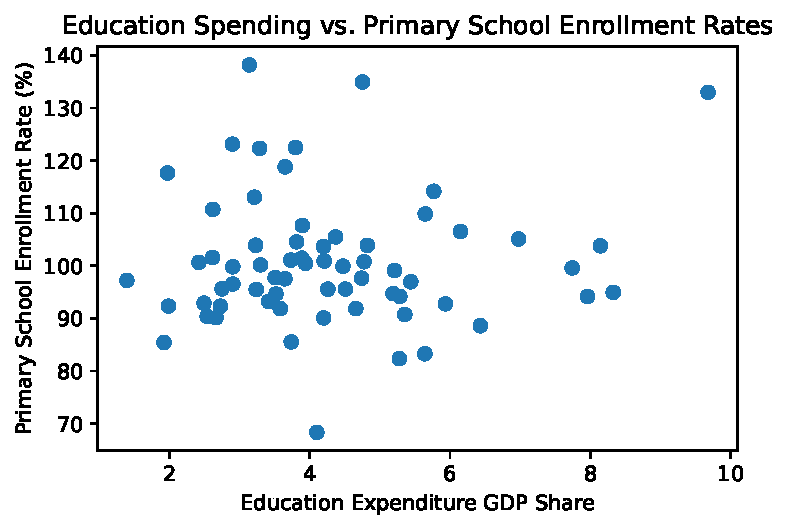
\includegraphics{assignment5_files/figure-pdf/cell-4-output-2.pdf}

\emph{Figure 1:} Relationship between share of GDP and primary school
enrollment {[}source{]}
(https://databank.worldbank.org/source/world-development-indicators).

\begin{Shaded}
\begin{Highlighting}[]
\NormalTok{plt.hist(wdi[}\StringTok{"adult\_literacy\_rate"}\NormalTok{])}
\NormalTok{plt.xlabel(}\StringTok{"Adult Literacy Rate (\%)"}\NormalTok{)}
\NormalTok{plt.ylabel(}\StringTok{"Frequency"}\NormalTok{)}
\NormalTok{plt.title(}\StringTok{"Distribution of Adult Literacy Rates"}\NormalTok{)}
\end{Highlighting}
\end{Shaded}

\begin{verbatim}
Text(0.5, 1.0, 'Distribution of Adult Literacy Rates')
\end{verbatim}

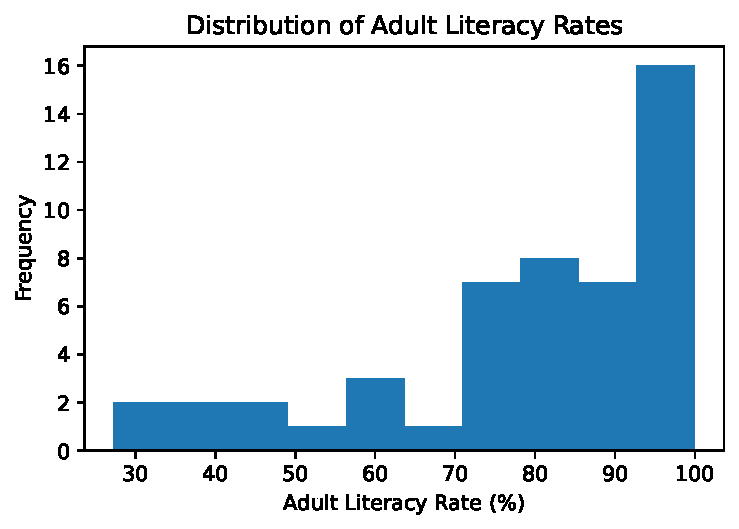
\includegraphics{assignment5_files/figure-pdf/cell-5-output-2.pdf}

\emph{Figure 2:} Distribution of adult literacy rates {[}source{]}
(https://databank.worldbank.org/source/world-development-indicators).

\subsection{Tables}\label{tables}

\begin{longtable}[]{@{}
  >{\raggedright\arraybackslash}p{(\columnwidth - 6\tabcolsep) * \real{0.4853}}
  >{\raggedright\arraybackslash}p{(\columnwidth - 6\tabcolsep) * \real{0.2353}}
  >{\raggedleft\arraybackslash}p{(\columnwidth - 6\tabcolsep) * \real{0.1324}}
  >{\centering\arraybackslash}p{(\columnwidth - 6\tabcolsep) * \real{0.1471}}@{}}
\toprule\noalign{}
\begin{minipage}[b]{\linewidth}\raggedright
Indicator
\end{minipage} & \begin{minipage}[b]{\linewidth}\raggedright
Mean (sd)
\end{minipage} & \begin{minipage}[b]{\linewidth}\raggedleft
Minimum
\end{minipage} & \begin{minipage}[b]{\linewidth}\centering
Maximum
\end{minipage} \\
\midrule\noalign{}
\endhead
\bottomrule\noalign{}
\endlastfoot
Adult Literacy Rate & 79.57\% (19.37\%) & 19.37\% & 99.99\% \\
Primary School Enrollment Rate & 100.87\%(12.04\%) & 64.40\% &
138.19\% \\
Education Expenditure GDP Share & 4.22\%(2.07\%) & 1.02\% & 16.58\% \\
\end{longtable}

\subsection{Bibliography}\label{bibliography}




\end{document}
